\chapter{System Modeling}
\label{sec:system_modeling}

\section{Use Case Diagram}
The use case model focuses on the implemented user-facing workflows that are most central to AutoReturn: unified message handling, assisted reply generation, voice-supported interaction, event extraction, and controlled attachment support.
\begin{figure}[htbp]
  \centering
  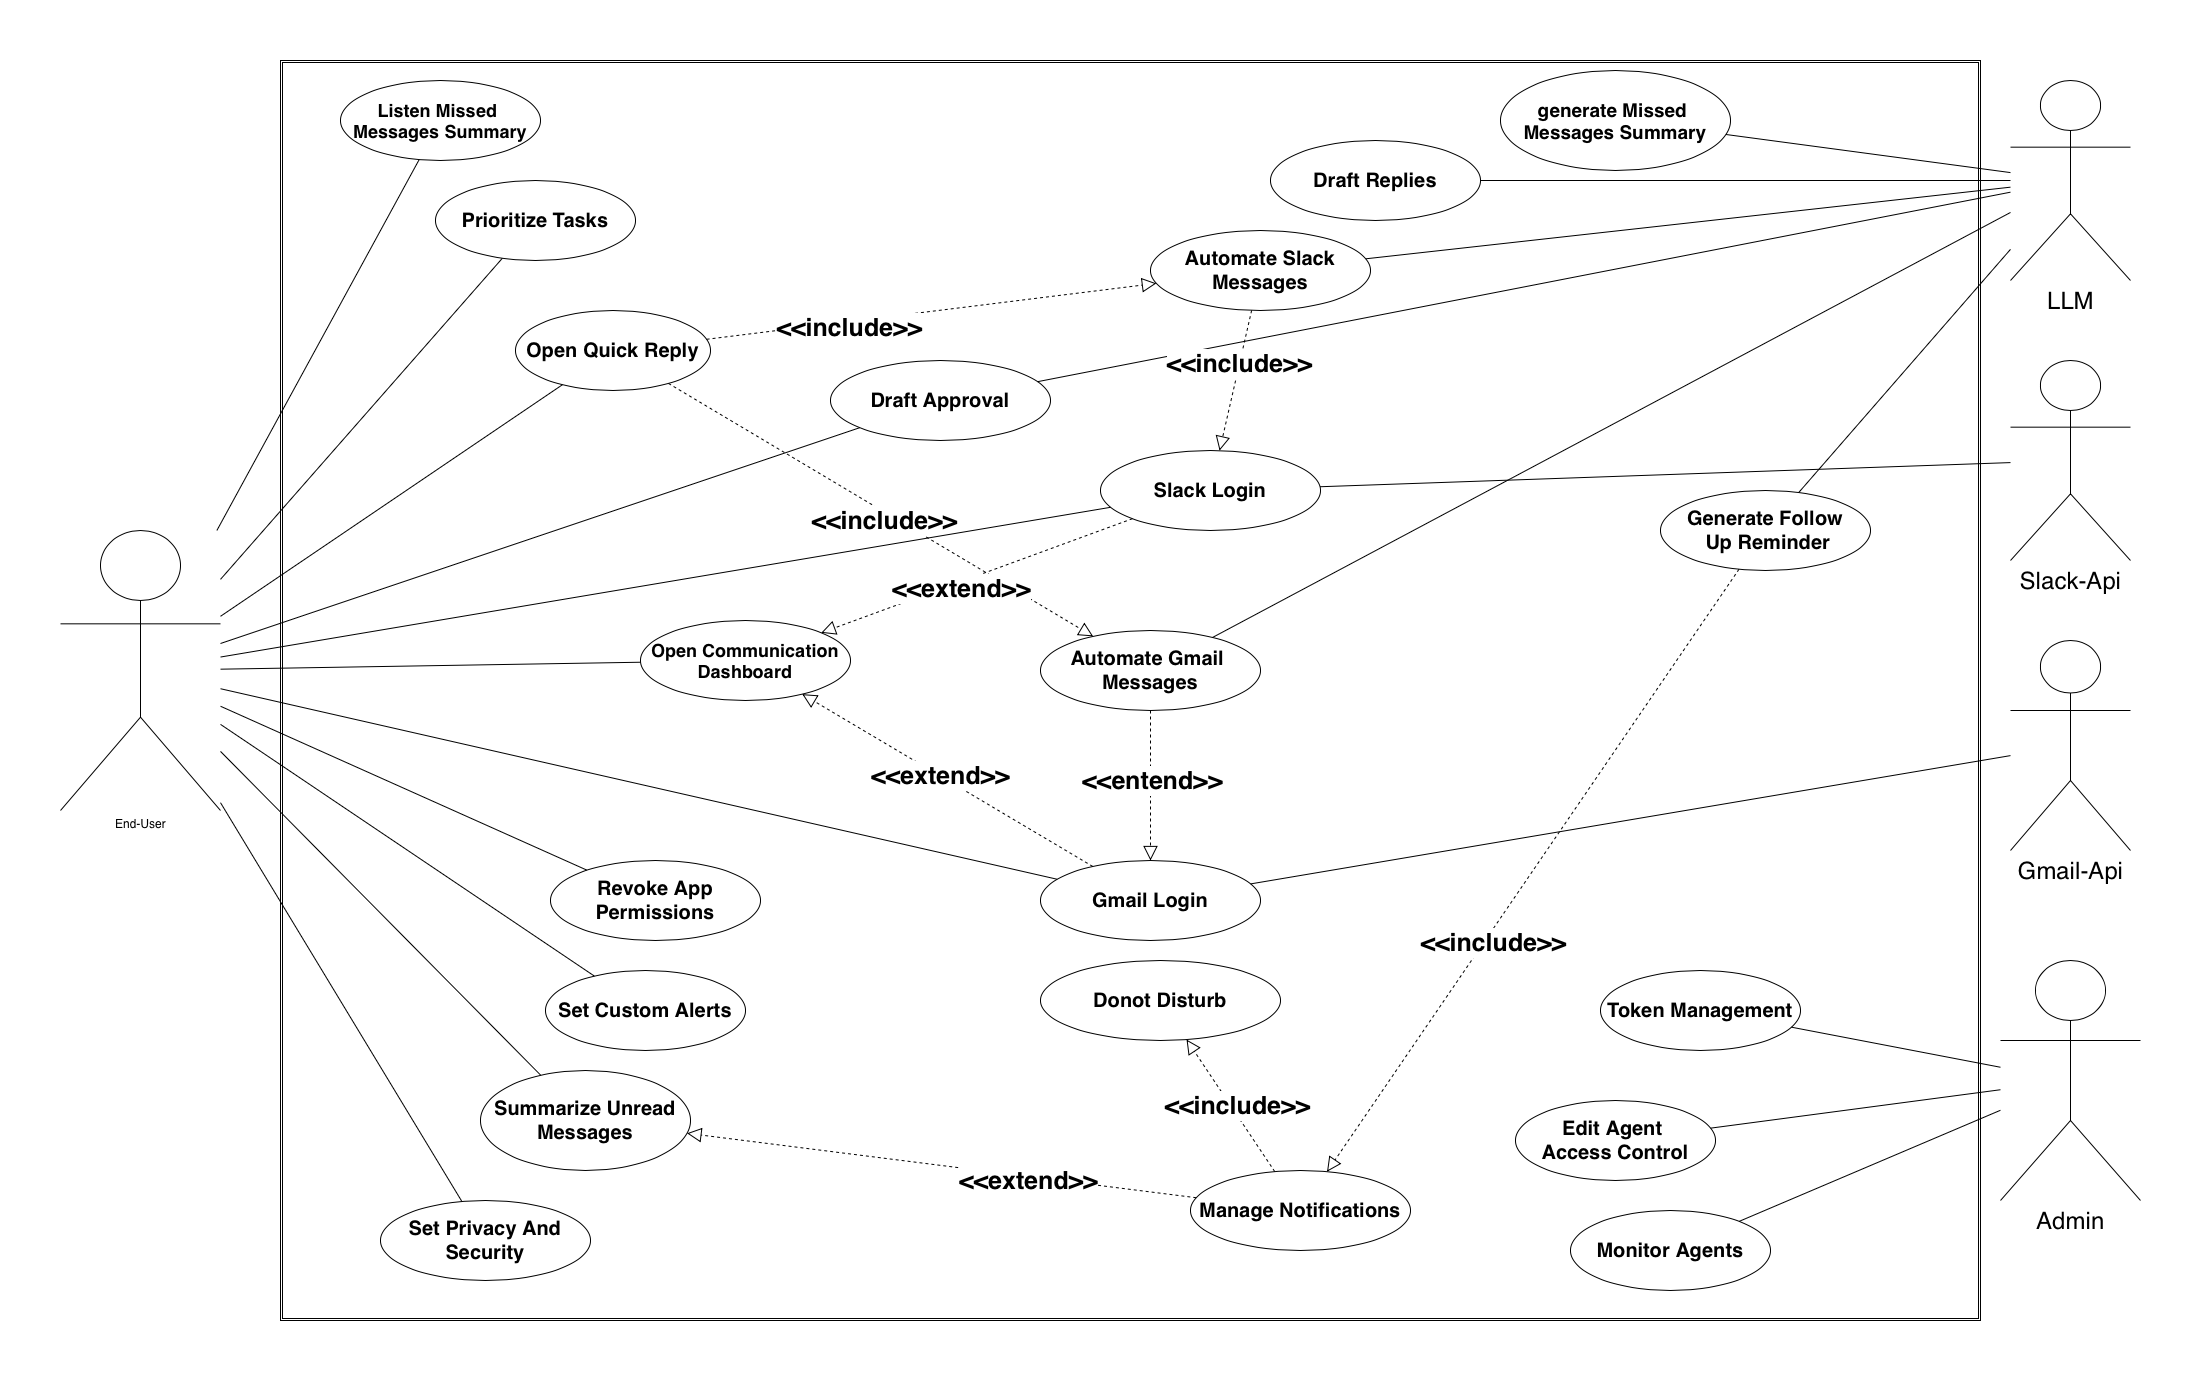
\includegraphics[width=\textwidth, height=0.83\textheight, keepaspectratio]{Figures/Usecase_Diagram.png}
  \caption[Use Case Diagram]{AutoReturn Use Case Diagram}
\end{figure}
\FloatBarrier

This diagram is intentionally centered on the practical behaviors that were implemented and tested in the final prototype. It avoids speculative functions and instead emphasizes the workflows that connect platform integration, assisted decision support, and user-controlled automation.

\section{Use Case Descriptions}
The following use cases describe the main user-facing workflows supported by the final AutoReturn prototype. Together, they show how the desktop interface, orchestration layer, and supporting services cooperate to produce controlled communication assistance.

\subsection{UC-01: Unified Inbox Management}
\textbf{Actor:} User \\
\textbf{Description:} The user views and manages consolidated messages from Gmail and Slack through a unified interface. \\
\textbf{Preconditions:} Gmail and Slack accounts are connected and authenticated. \\
\textbf{Main Flow:}
\begin{enumerate}
    \item The user opens the AutoReturn application.
    \item The system retrieves messages from connected platforms.
    \item The system displays the unified inbox with message summaries and priority indicators.
    \item The user filters, sorts, or searches messages.
    \item The user opens a message and decides whether to review, summarize, or respond.
\end{enumerate}
\textbf{Postconditions:} Messages remain available in the unified inbox and subsequent actions can be routed through the same workflow.

This use case represents the central entry point of the system because many other workflows begin from a message selected in the unified inbox. It therefore captures the practical value of AutoReturn as a workspace rather than as a set of disconnected features.

\subsection{UC-02: Draft and Reply Assistance}
\textbf{Actor:} User, System \\
\textbf{Description:} The system generates contextual response drafts and applies configured reply policies before any message is sent. \\
\textbf{Preconditions:} Draft generation or reply support is enabled for the connected platform. \\
\textbf{Main Flow:}
\begin{enumerate}
    \item The system receives or loads a message.
    \item The priority classification module determines the urgency level of the message.
    \item A model-backed service generates a contextual response draft.
    \item The tone preference module adjusts the response style.
    \item The system checks policy rules such as review-first mode, DND, and sender allowlists.
    \item The system either saves the draft for review or completes the reply path permitted by policy.
    \item The action is logged for user review.
\end{enumerate}
\textbf{Postconditions:} A response draft or controlled reply action is produced and recorded.

This use case is important because it combines several of the project’s core ideas in one flow: model-assisted drafting, tone adjustment, and policy-based control. It also shows how the system preserves user oversight when communication actions carry greater risk.

\subsection{UC-03: Voice-Assisted Control}
\textbf{Actor:} User \\
\textbf{Description:} The user interacts with the system using voice-assisted controls where supported by the current implementation. \\
\textbf{Preconditions:} A microphone is available and voice interaction features are enabled. \\
\textbf{Main Flow:}
\begin{enumerate}
    \item The user activates the voice interaction feature.
    \item The system accepts a spoken command.
    \item The command is converted into text for processing.
    \item The system interprets the requested action.
    \item The system executes the requested operation.
    \item The system provides feedback to the user.
\end{enumerate}
\textbf{Postconditions:} The requested command is processed and the user is informed of the result.

Although voice support is not the sole focus of the final prototype, it remains relevant as a supporting interaction pathway. This use case therefore reflects the intended role of voice as an extension of the desktop workflow rather than a separate conversational product.

\subsection{UC-04: Task Extraction and Management}
\textbf{Actor:} User, System \\
\textbf{Description:} The system analyzes incoming messages and extracts actionable information such as events, deadlines, or follow-up items for user review. \\
\textbf{Preconditions:} Extraction services are enabled for the current message workflow. \\
\textbf{Main Flow:}
\begin{enumerate}
    \item The system processes an incoming message.
    \item Model-assisted extraction analyzes the message for events, deadlines, or requested actions.
    \item The system structures the extracted information for review.
    \item The user reviews, edits, or confirms the extracted result.
    \item When relevant, the system prepares an exportable event or follow-up artifact.
\end{enumerate}
\textbf{Postconditions:} Actionable information is extracted and prepared for later use.

This workflow demonstrates how AutoReturn moves beyond message viewing and reply generation into actionable interpretation. It is particularly important for event handling, follow-up support, and other productivity-oriented extensions of communication analysis.

\subsection{UC-05: File Attachment Automation}
\textbf{Actor:} User, System \\
\textbf{Description:} The system identifies and attaches relevant files to outgoing responses based on user requests and file-matching logic. \\
\textbf{Preconditions:} File attachment automation is enabled and authorized directories are configured. \\
\textbf{Main Flow:}
\begin{enumerate}
    \item The system detects a file request in the outgoing message.
    \item The system searches configured directories for matching files.
    \item If a single match is found, the file is attached automatically.
    \item If multiple matches are found, the user is prompted to select the correct file.
    \item The selected file is attached to the outgoing response.
\end{enumerate}
\textbf{Postconditions:} The outgoing message is prepared with the correct file attachment.

This use case also illustrates the project’s emphasis on cautious automation. Rather than attaching files aggressively, the system is designed to stop and request confirmation when ambiguity would reduce trust or increase error risk.

\section{Activity Diagrams}
\noindent The activity diagrams summarize the highest-level workflows implemented in the current prototype. They illustrate control flow rather than every internal service call.
\Needspace{0.42\textheight}
\subsection{Overall System Activity}
\begin{figure}[H]
  \centering
  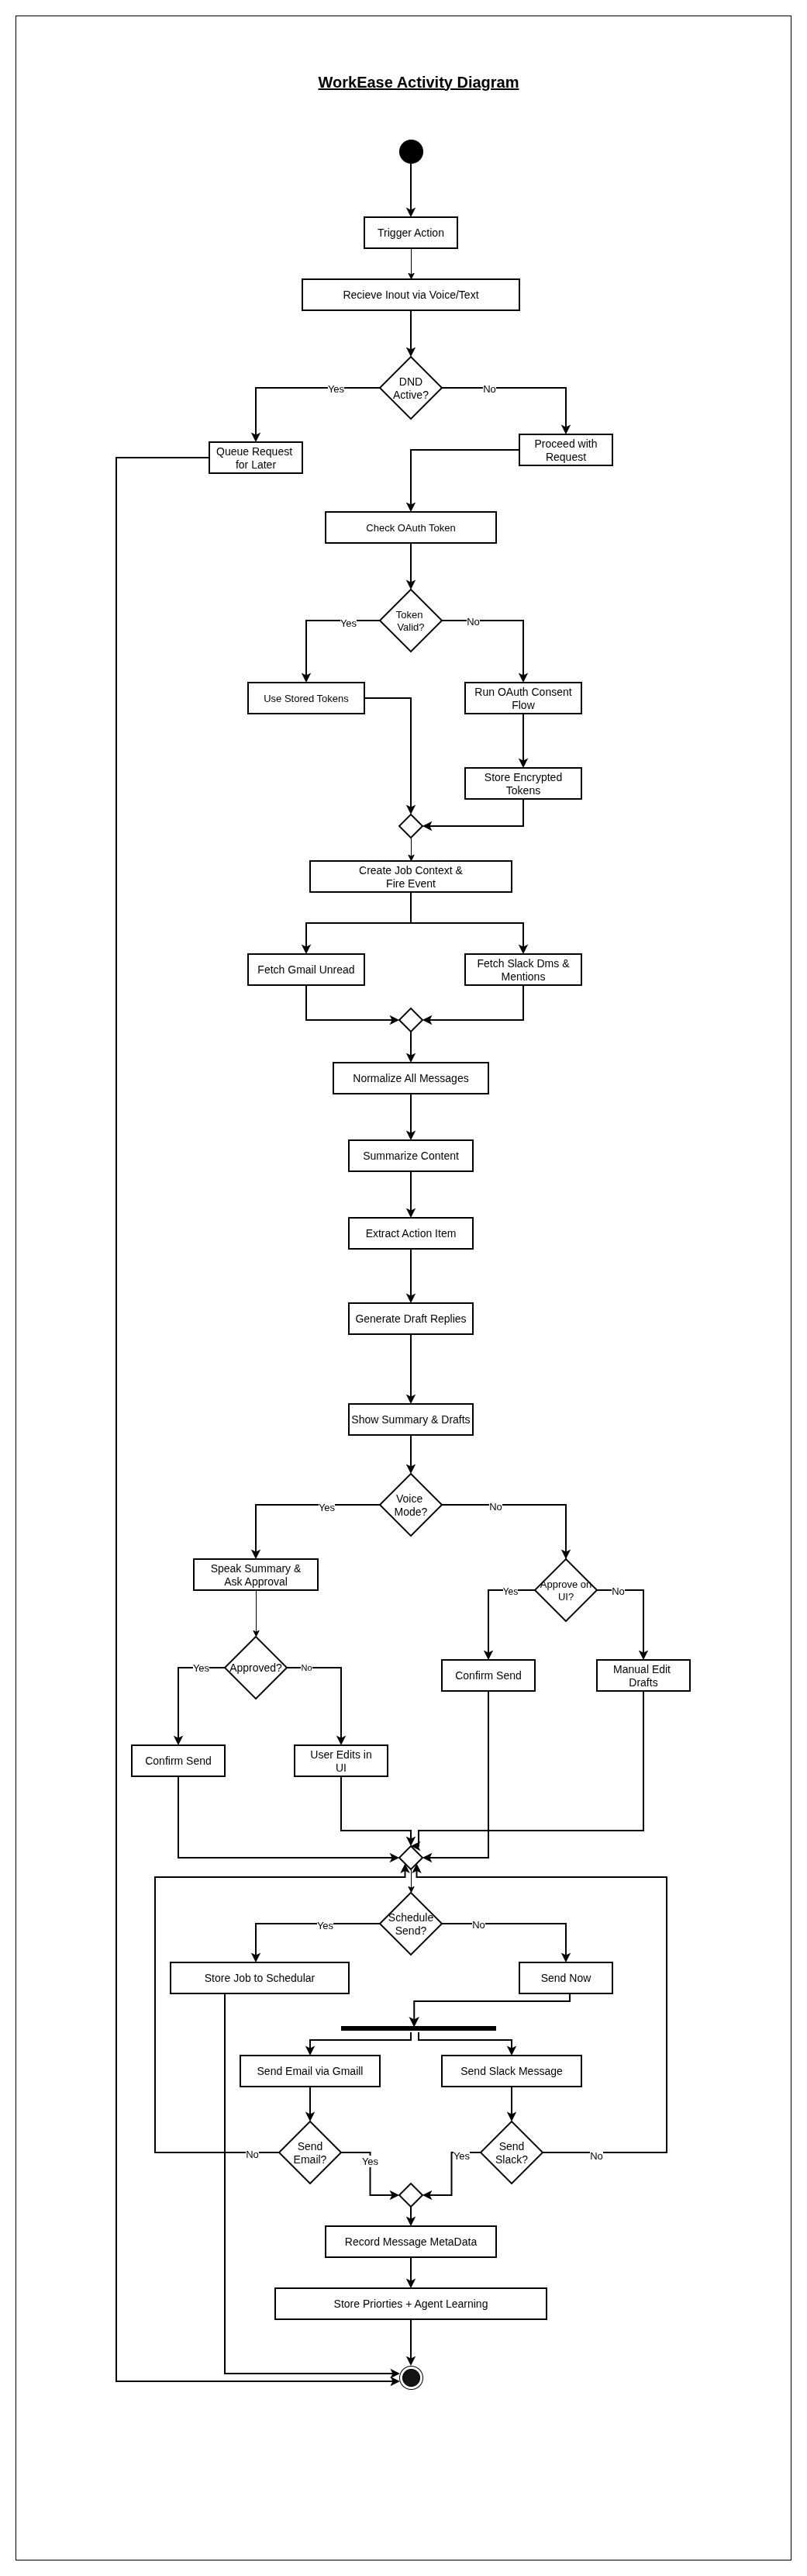
\includegraphics[width=\textwidth, height=0.76\textheight, keepaspectratio]{Figures/Complete_Activity_Diagram.png}
  \caption[System Activity Diagram]{Overall System Activity Diagram}
\end{figure}
\FloatBarrier

The overall activity diagram is useful because it compresses the major workflow stages into one view, from message intake to assisted action. It helps explain how the system coordinates retrieval, analysis, policy checks, and output preparation as one connected flow.

\Needspace{0.38\textheight}
\subsection{Activity 1: Voice-Based Interaction and Control}
\begin{figure}[H]
  \centering
  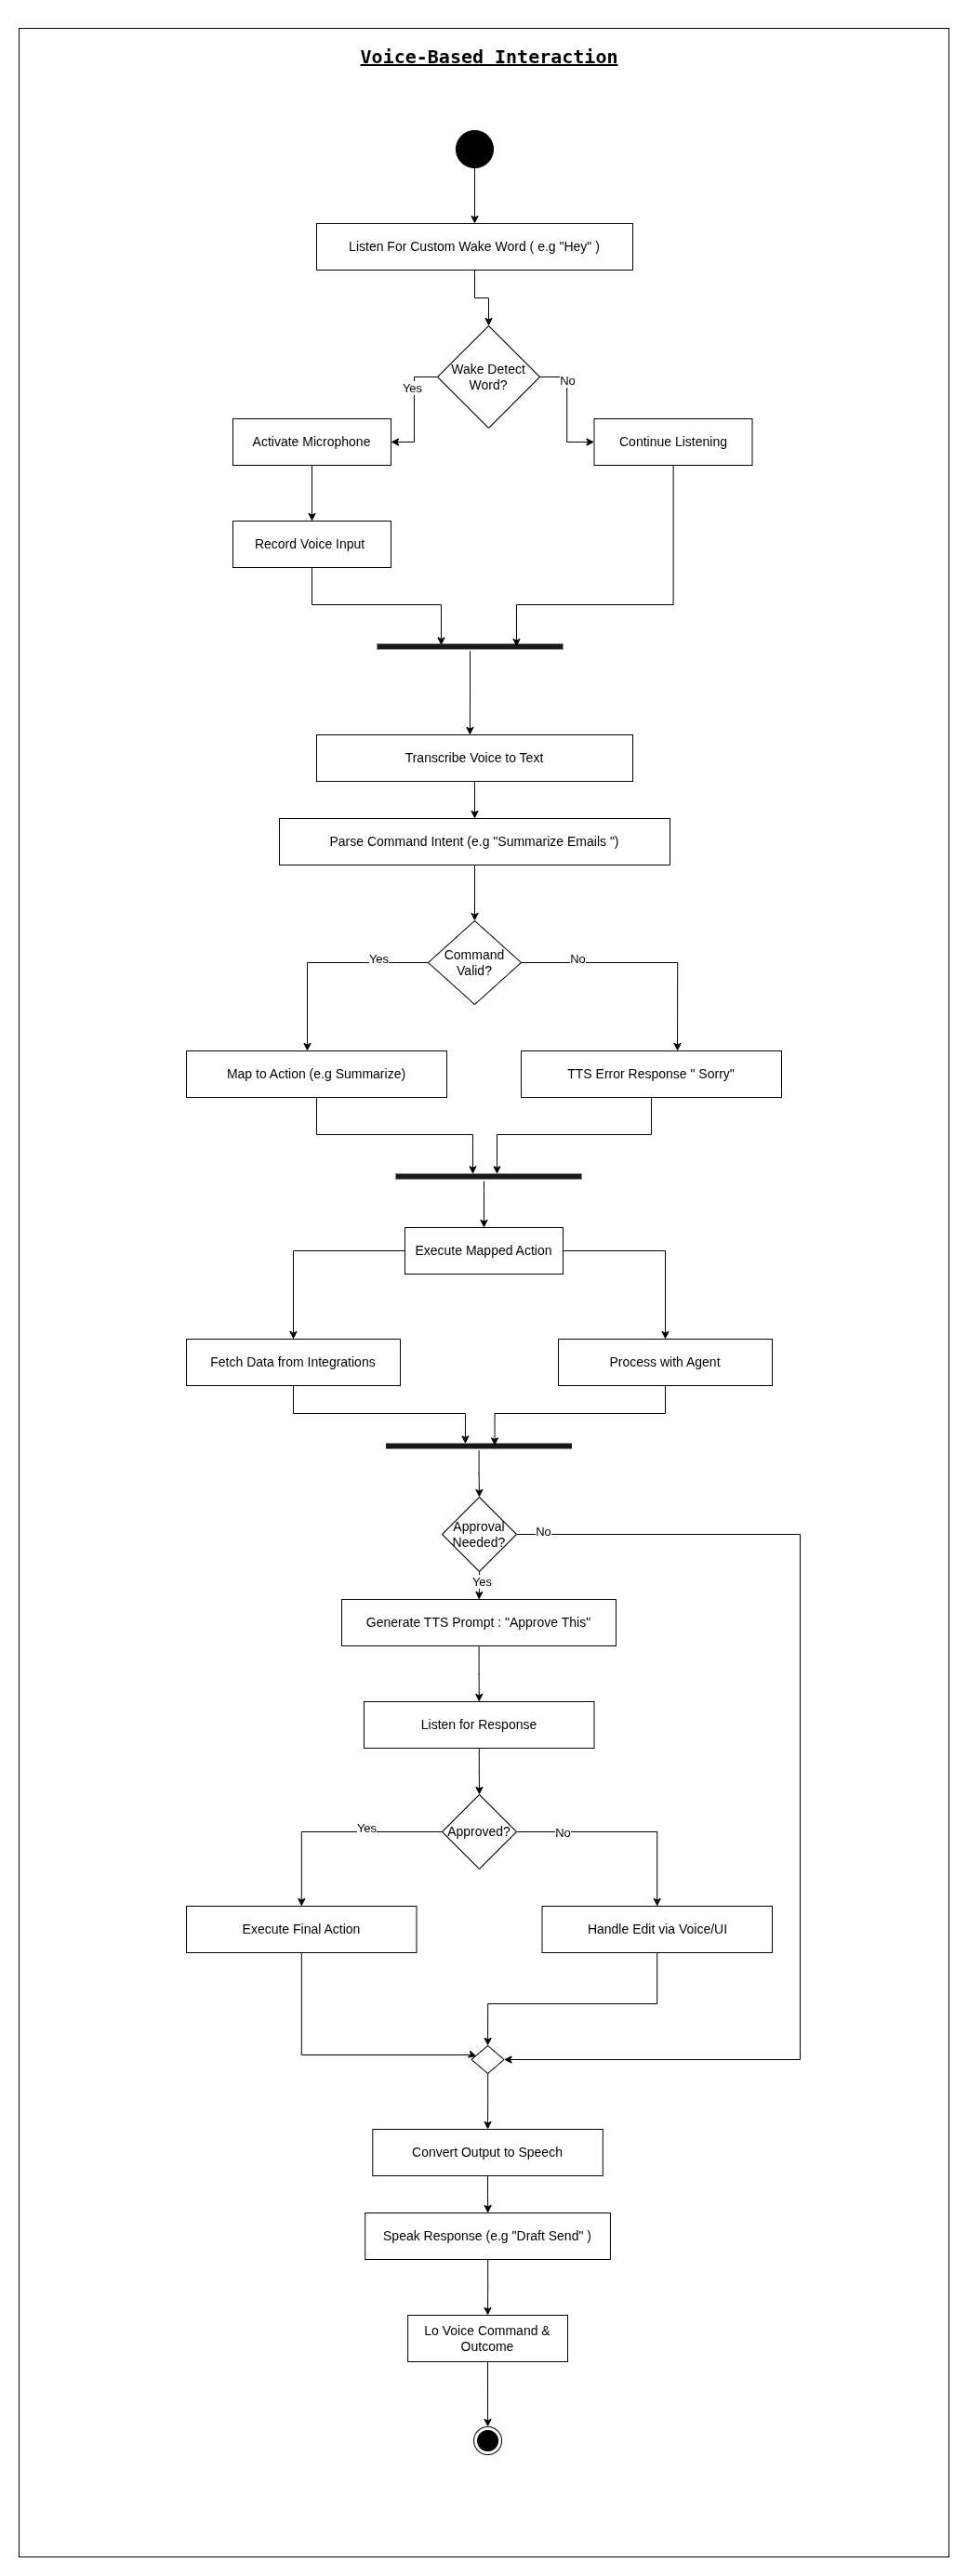
\includegraphics[width=\textwidth, height=0.72\textheight, keepaspectratio]{Figures/Activity_1_Voice_Based_Interaction.png}
  \caption[Voice Interaction Activity Diagram]{Voice Interaction Activity Diagram}
\end{figure}
\FloatBarrier

This activity emphasizes the narrower but still meaningful role of voice support in the final system. It shows that voice is treated as a controlled trigger for supported actions rather than as the sole interaction model.

\Needspace{0.38\textheight}
\subsection{Activity 2: Smart Email and Message Automation}
\begin{figure}[H]
  \centering
  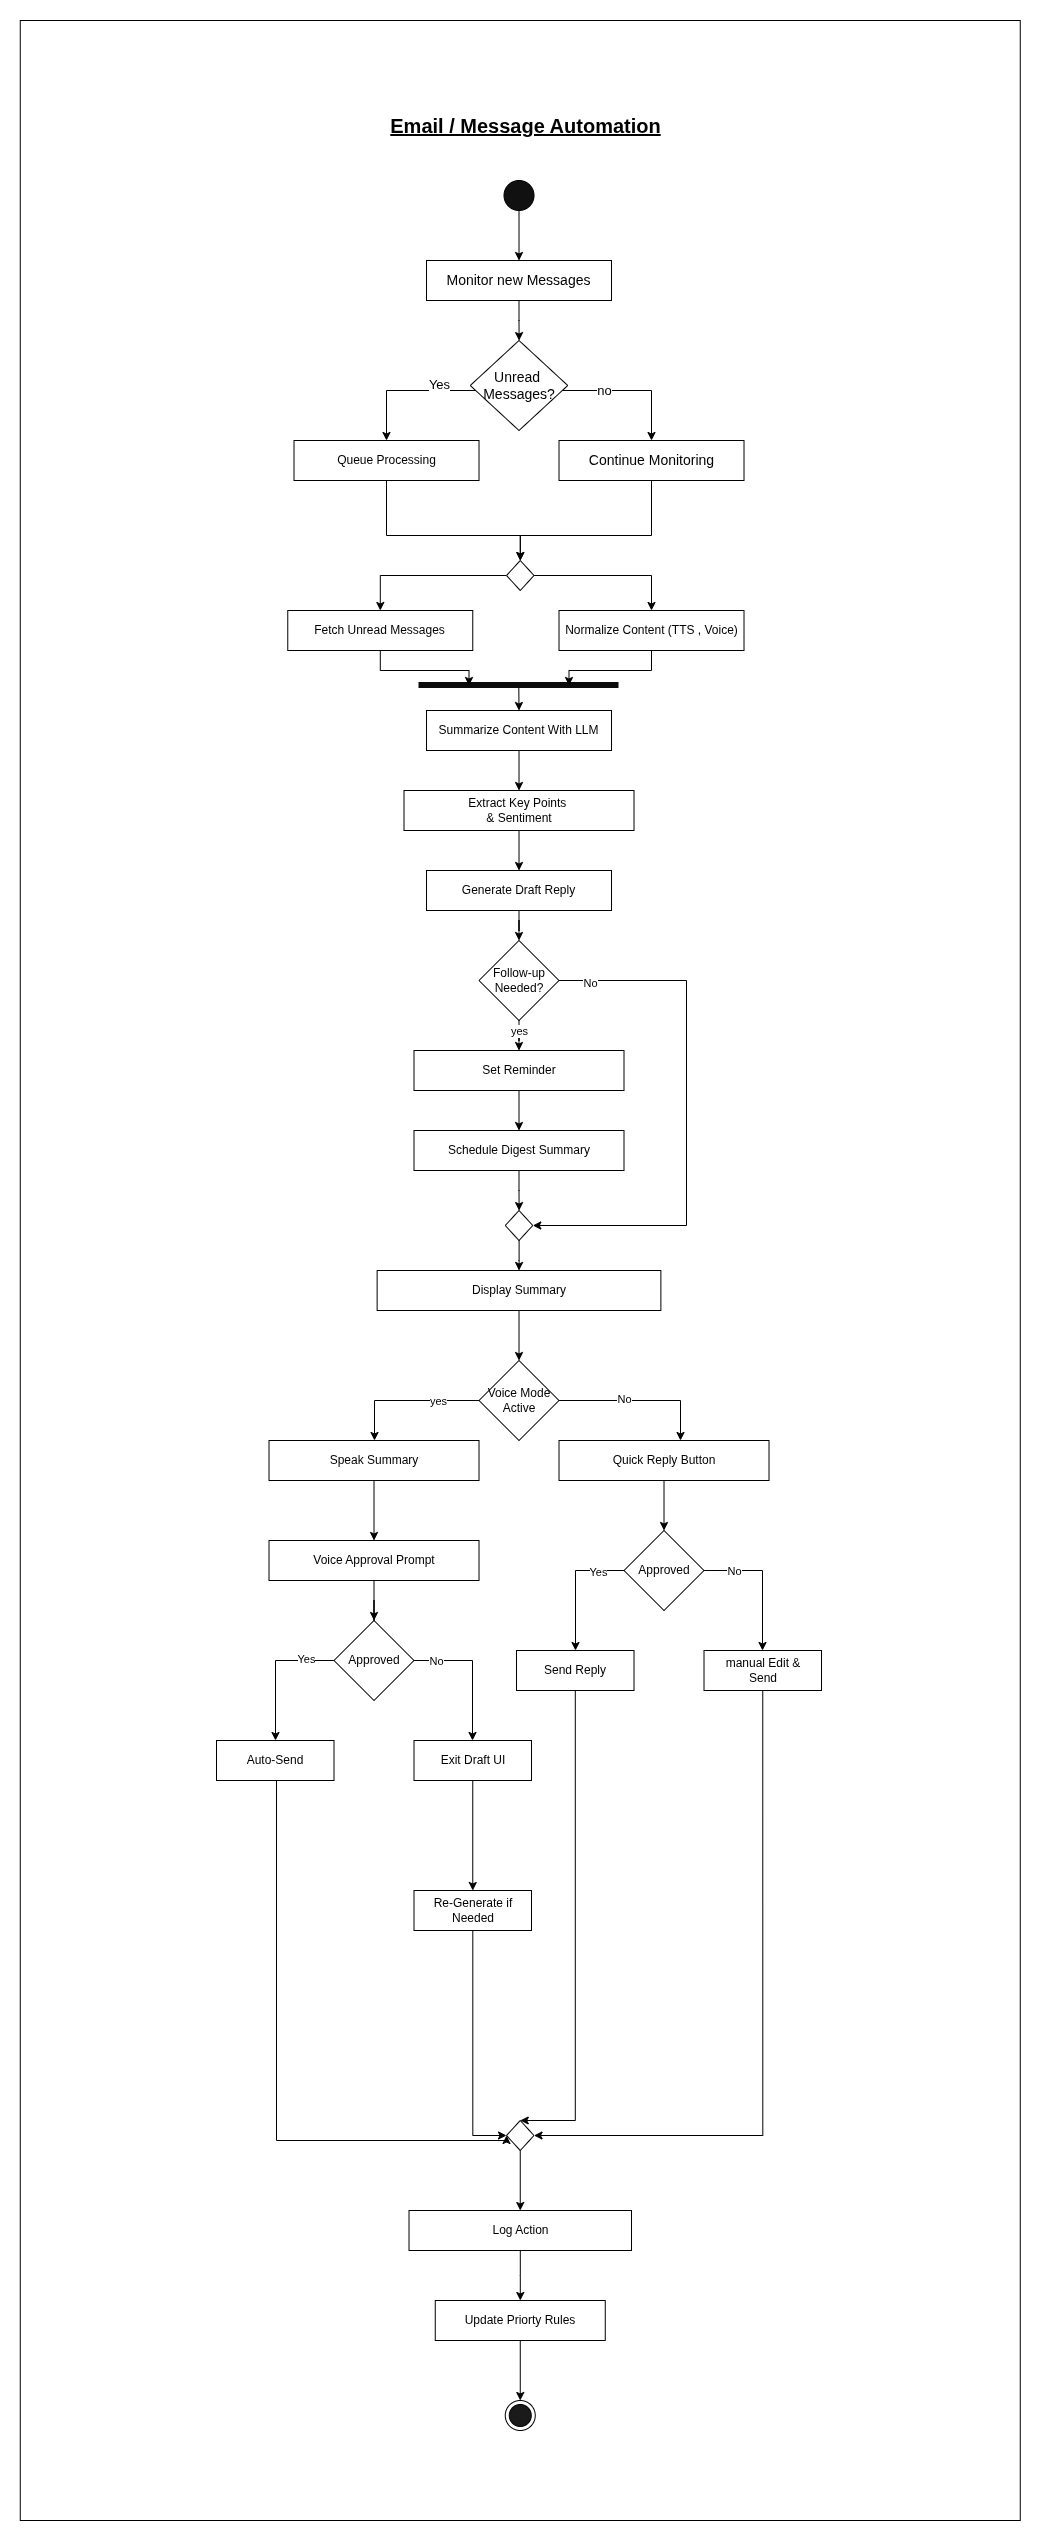
\includegraphics[width=\textwidth, height=0.72\textheight, keepaspectratio]{Figures/Activity_2_Email_Message_Automation.png}
  \caption[Smart Automation Activity Diagram]{Smart Email and Message Automation Activity Diagram}
\end{figure}
\FloatBarrier

This diagram is important because it captures the project’s most representative intelligent workflow: receiving a message, analyzing it, generating support artifacts, and applying user-governed response rules. It therefore reflects the practical center of the implementation.

\Needspace{0.36\textheight}
\subsection{Activity 3: Multi-App Integration and Authentication}
\begin{figure}[H]
  \centering
  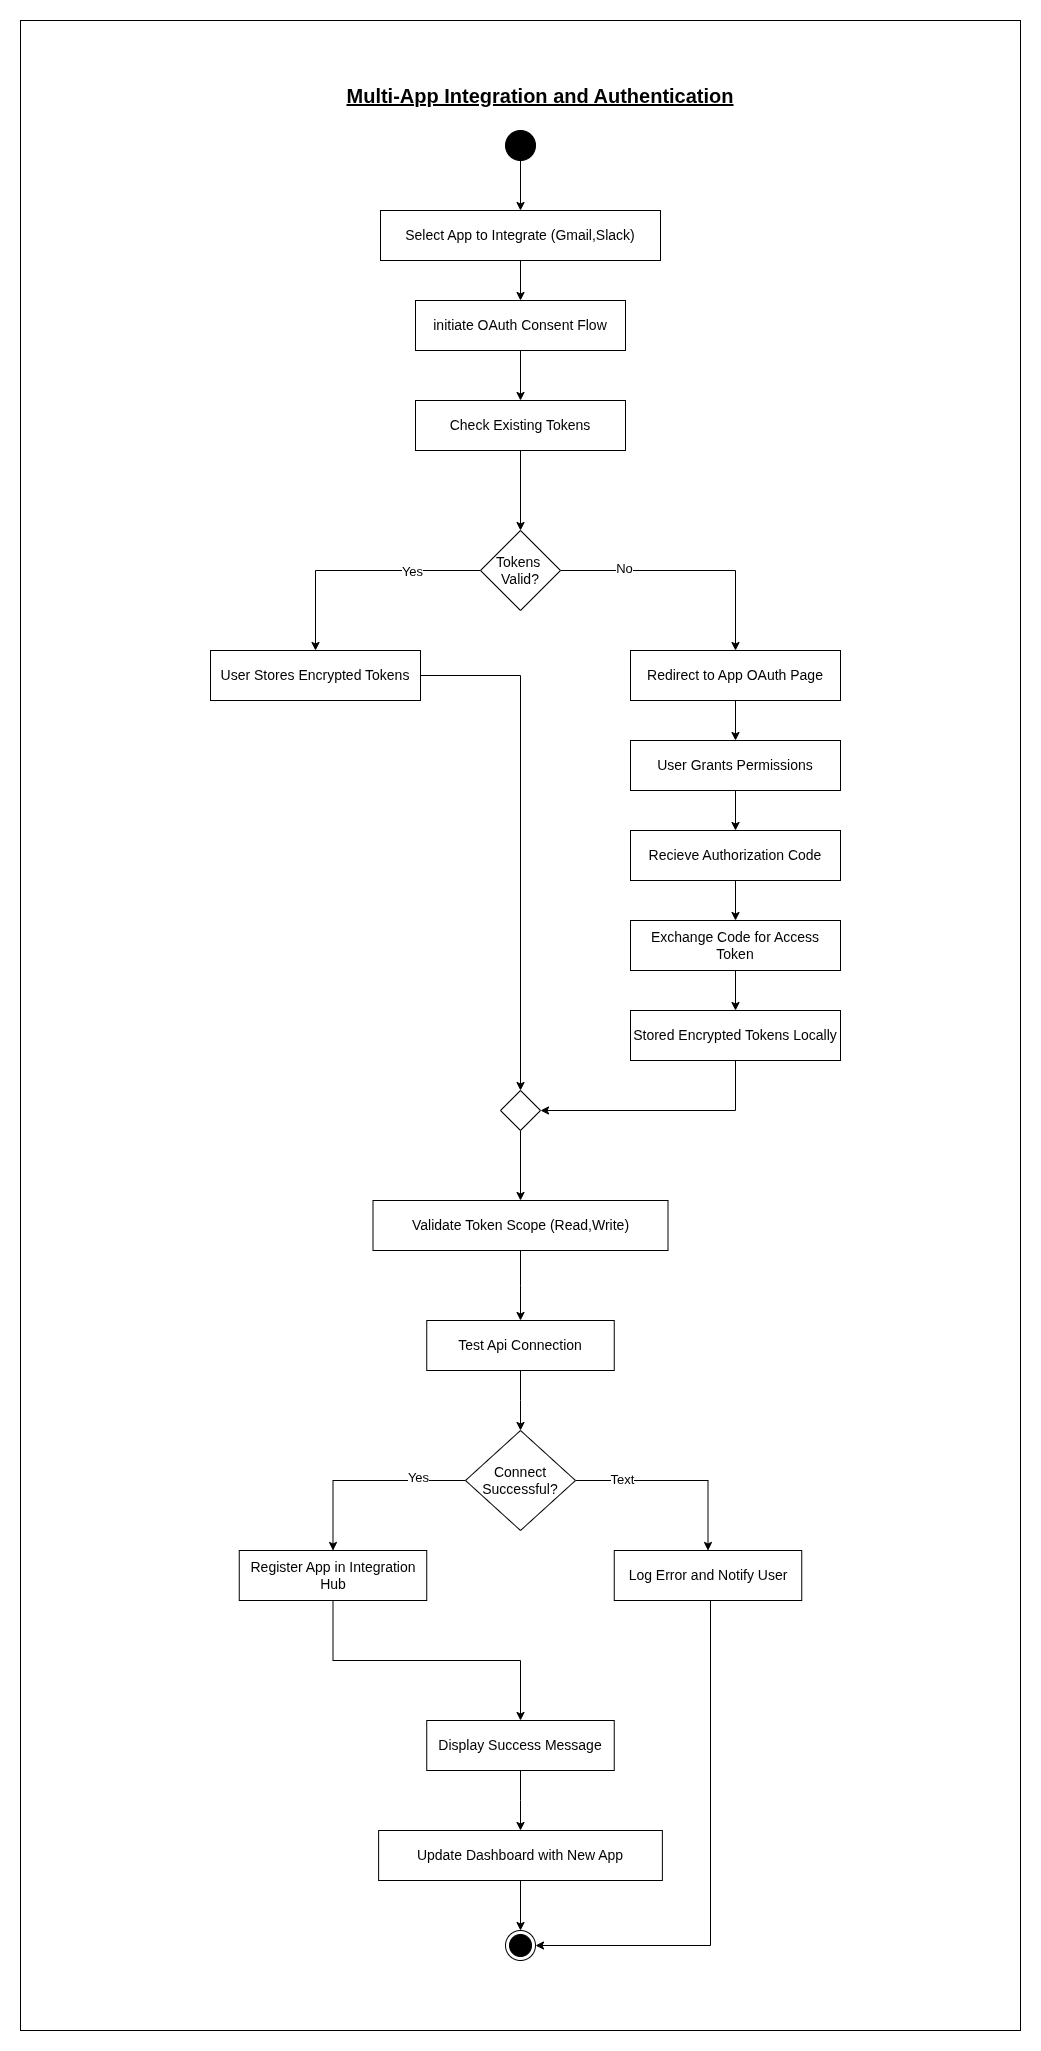
\includegraphics[width=\textwidth, height=0.70\textheight, keepaspectratio]{Figures/Activity_3_MultiApp_Integration.png}
  \caption[Multi-App Activity Diagram]{Multi-App Integration Activity Diagram}
\end{figure}
\FloatBarrier

The multi-app activity also highlights why the orchestrator-agent design was necessary. Different platforms must be normalized and coordinated before later intelligent services can operate consistently across them.

Together, these diagrams show that the system is organized around repeatable workflow stages rather than isolated feature calls. This process view is important for understanding how AutoReturn coordinates retrieval, analysis, user review, and controlled action.

\section{Component Diagram}
\noindent Figure 4.6 presents the major implementation blocks and their interaction boundaries.
\begin{figure}[htbp]
  \centering
  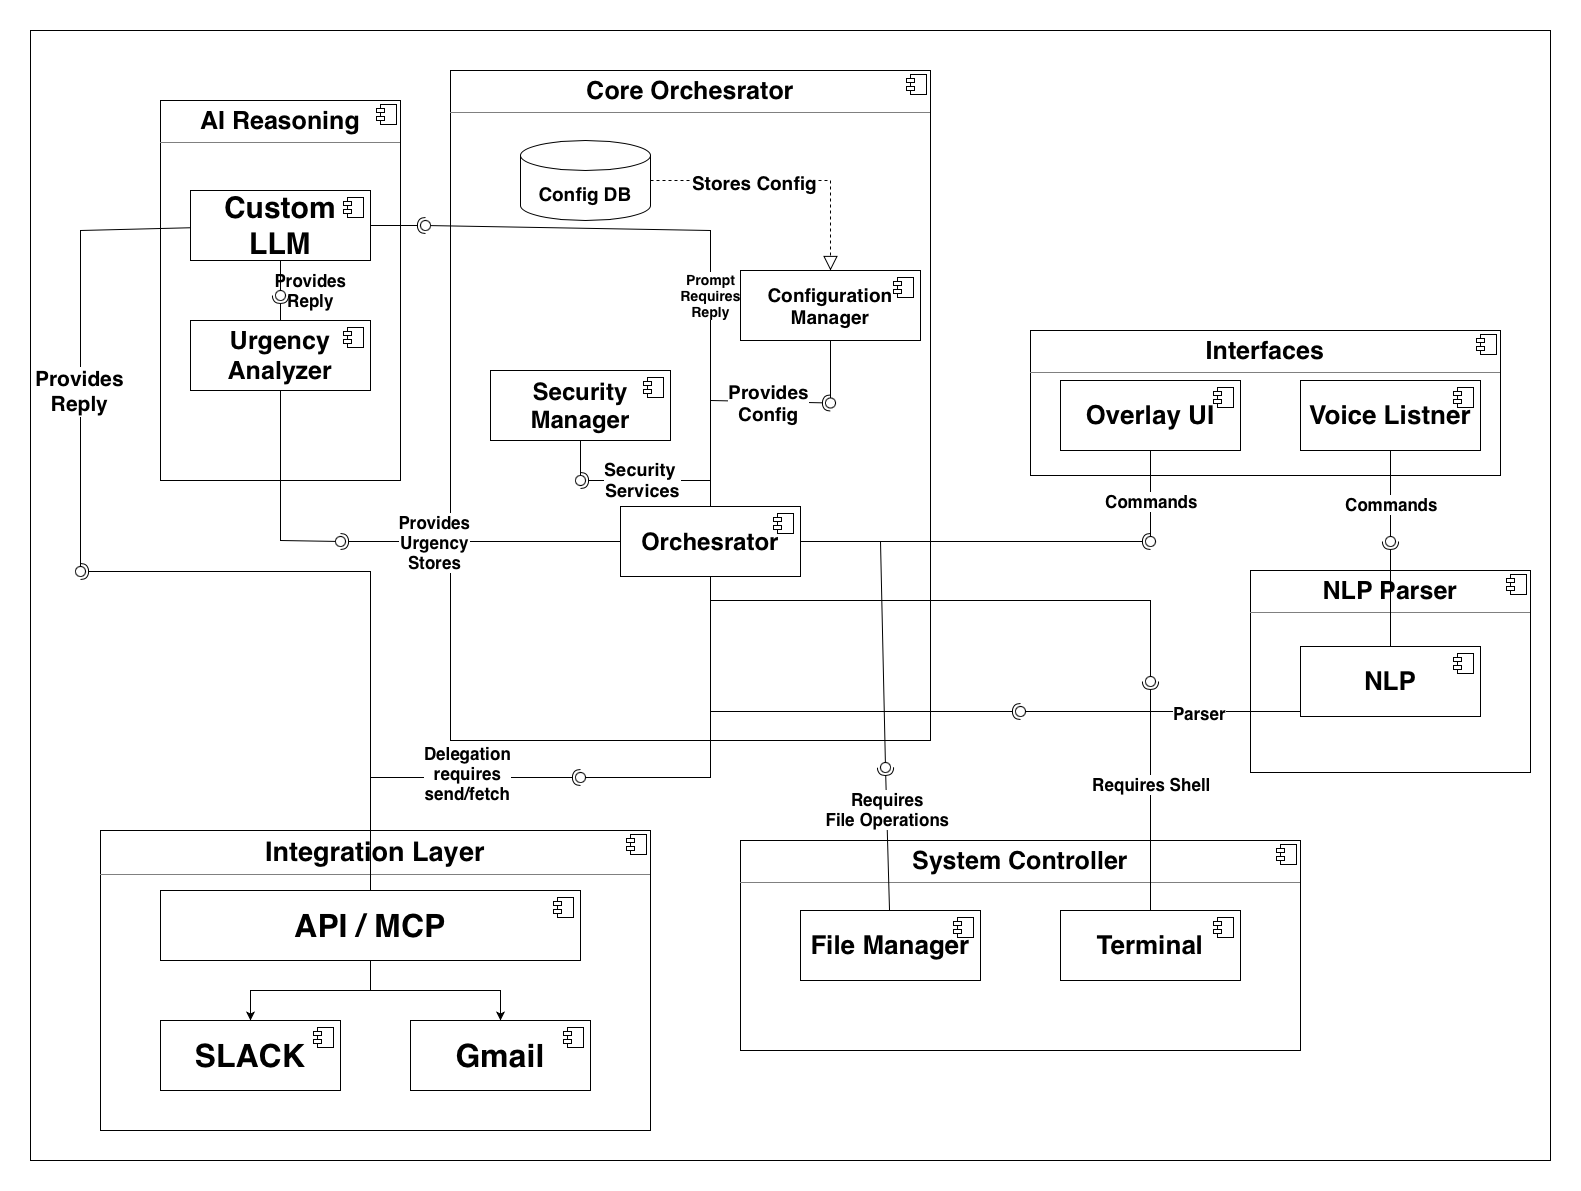
\includegraphics[width=\textwidth, height=0.90\textheight, keepaspectratio]{Figures/Component.png}
  \caption[Component Diagram]{AutoReturn Component Diagram}
\end{figure}
\FloatBarrier

The component view complements the earlier behavioral diagrams by showing how those workflows are distributed across the main software units. It also highlights the separation between interface concerns, orchestration logic, platform agents, and supporting backend services.

\section{Architecture Diagram}
\noindent The architecture diagram emphasizes the final desktop-oriented structure: a PySide6 user interface, an orchestration layer, platform agents, and shared processing services.
\begin{figure}[!htbp]
    \centering
    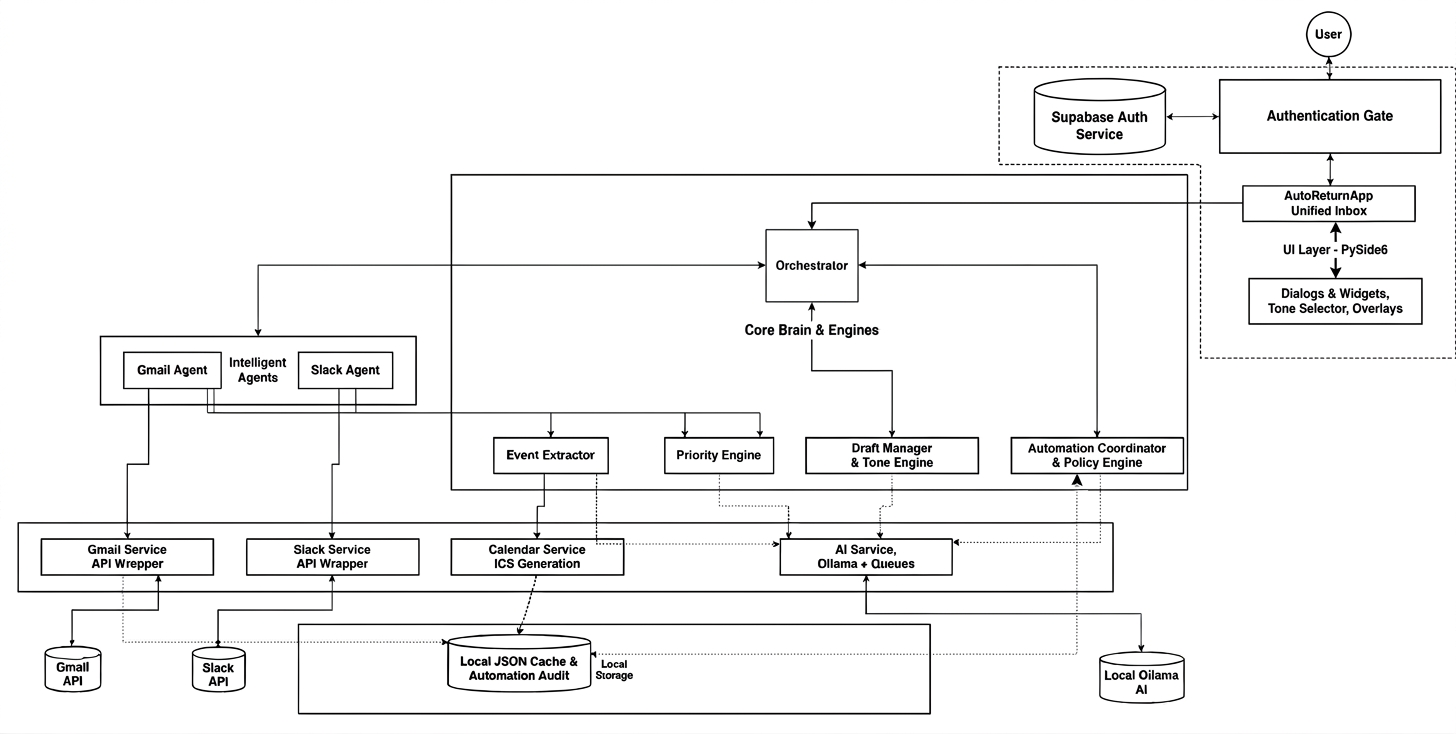
\includegraphics[width=1.08\textwidth]{Figures/Architecture5.png}
    \caption[System Architecture]{AutoReturn System Architecture}
    \label{fig:architecture}
\end{figure}

This architectural perspective is especially useful because AutoReturn depends on coordination between several subsystems rather than on a single processing pipeline. The diagram therefore reinforces the modular design rationale introduced in the earlier chapters.

\section{Wireframes}
\noindent The wireframes in this section present the intended interaction layout of the AutoReturn desktop interface. They complement the structural diagrams by showing how unified inbox navigation, assisted reply handling, notifications, and voice entry points were organized at the interface level.

\subsection{Unified Workspace Wireframe}
\begin{figure}[!htbp]
    \centering
    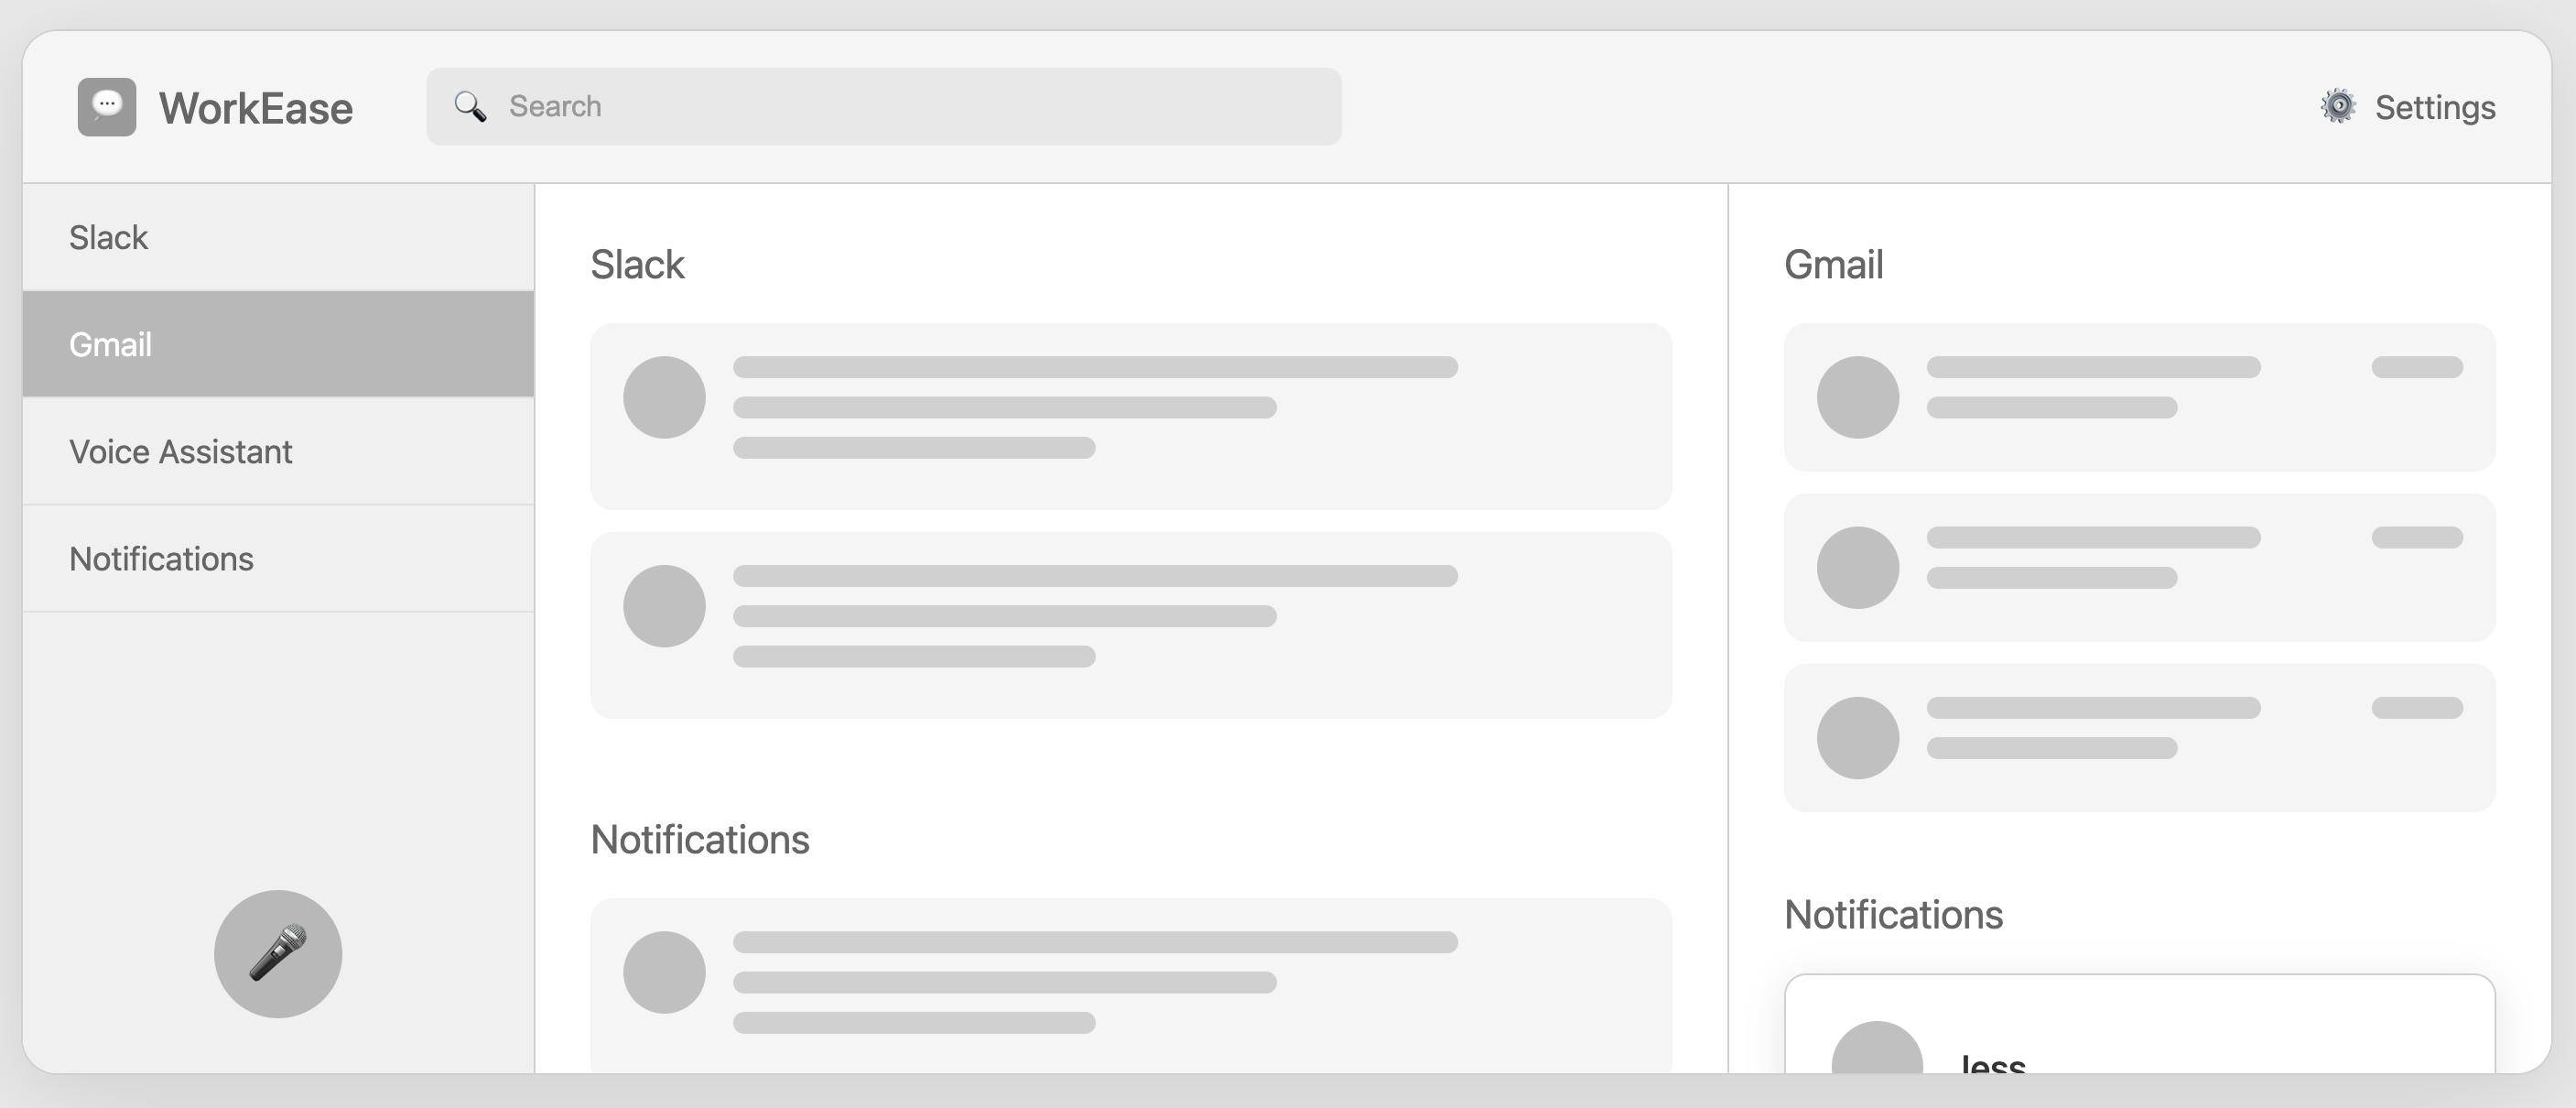
\includegraphics[width=1.03\textwidth]{Figures/Wireframe2.png}
\caption[Unified Workspace Wireframe]{AutoReturn Unified Workspace Wireframe}
\label{fig:wireframe_workspace}
\end{figure}

This wireframe helps show how the technical goals of unification, visibility, and assisted action are translated into one main working screen. It therefore provides an interface-level interpretation of the architectural and workflow diagrams presented earlier.

\subsection{Notification and Assisted Reply Wireframe}
\begin{figure}[!htbp]
    \centering
    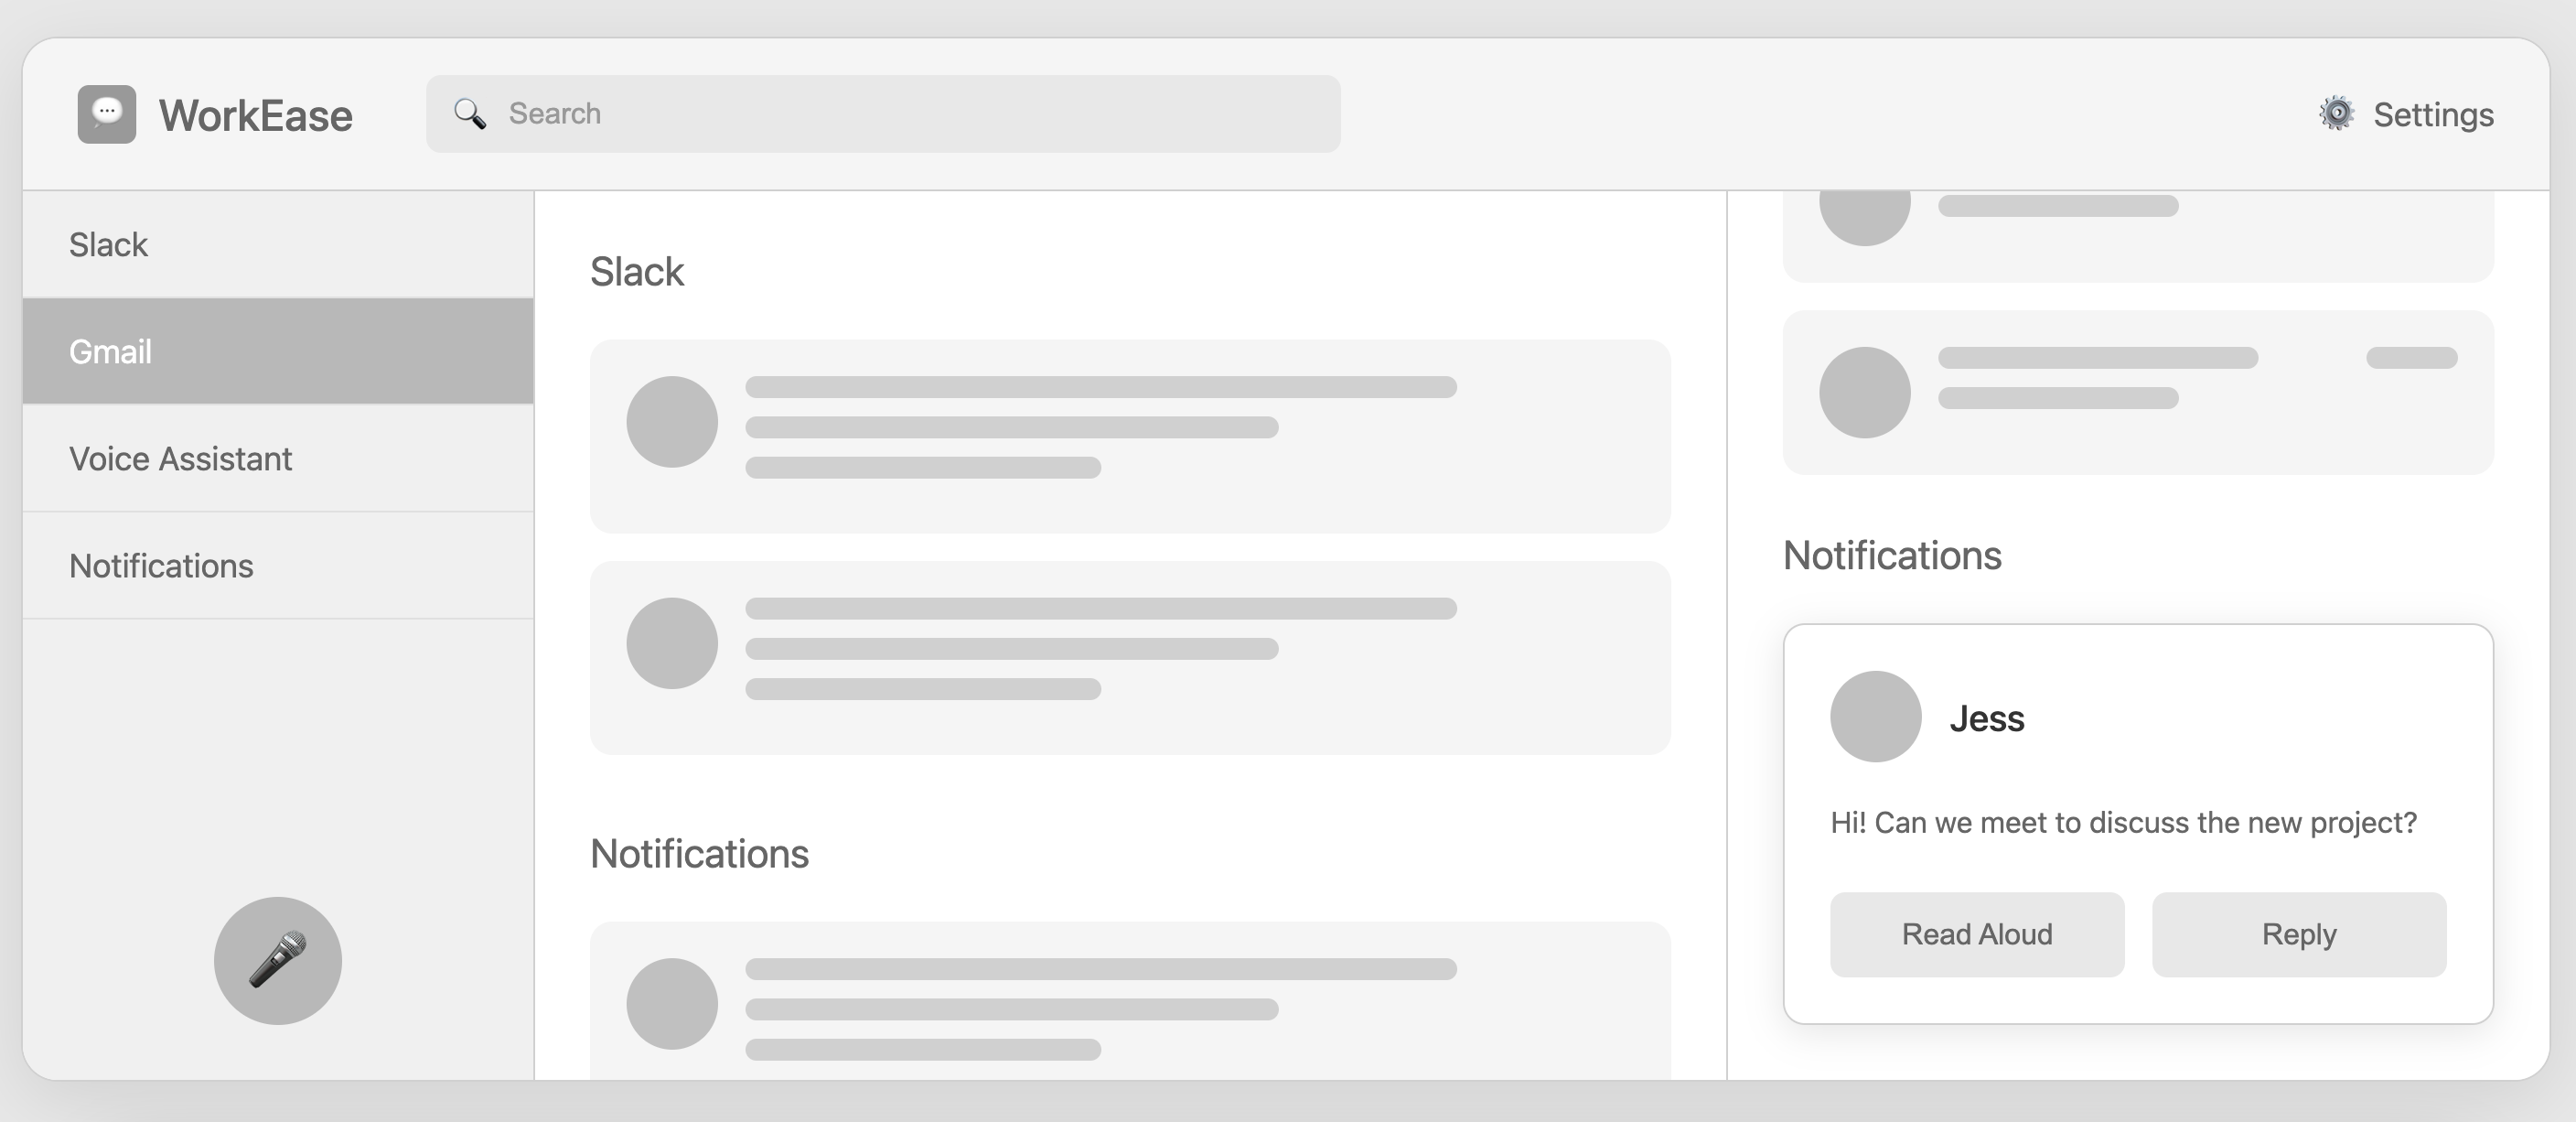
\includegraphics[width=1.03\textwidth]{Figures/wireframe1.png}
    \caption[Reply Assistant Wireframe]{Notification and Reply Wireframe}
    \label{fig:wireframe_reply}
\end{figure}

These wireframes are included to show how the technical architecture becomes visible to the user as a coherent workspace. They therefore bridge the gap between the abstract system model and the practical layout of the implemented interface.

\section{Modeling Discussion}
The modeling view presented in this chapter reflects the final prototype more accurately than the earlier concept-stage architecture. AutoReturn is best understood as a desktop system with a unified interface, an orchestration layer, platform agents, policy services, and model-assisted support components. The structural diagrams explain the underlying workflow, while the wireframes show how these functions are surfaced to the user in the desktop application.

Viewed together, the modeling artifacts provide a balanced description of the system from functional, behavioral, structural, and interface perspectives. This is more useful for the current project than a narrowly code-centric model because AutoReturn’s value lies in coordinated workflow behavior across multiple services.
